\documentclass[11pt,letterpaper]{article}

% Packages
\usepackage{amsmath,amssymb,amsthm}
\usepackage{mathtools}
\usepackage{microtype}
\usepackage{graphicx}
\usepackage{booktabs}
\usepackage{tikz}
\usetikzlibrary{shapes,arrows,positioning}
\usepackage{pgfplots}
\pgfplotsset{compat=1.18}
\usepackage[hidelinks]{hyperref}
\usepackage{geometry}
\usepackage{enumitem}

\geometry{margin=1in}

% Theorem environments (used for crisp accounting statements)
\newtheorem{theorem}{Theorem}[section]
\newtheorem{proposition}[theorem]{Proposition}
\newtheorem{corollary}[theorem]{Corollary}
\theoremstyle{definition}
\newtheorem{definition}[theorem]{Definition}
\theoremstyle{remark}
\newtheorem{remark}[theorem]{Remark}

% Custom commands
\newcommand{\R}{\mathbb{R}}
\newcommand{\N}{\mathbb{N}}
\newcommand{\defeq}{\coloneqq}
\newcommand{\TGA}{\mathrm{TGA}}
\newcommand{\NFA}{\mathrm{NFA}}

\setlist[itemize]{nosep,leftmargin=*}
\setlist[enumerate]{nosep,leftmargin=*}

\title{Stock-Flow Consistent Monetary Operations:\\
Sectoral Balances and Why ``Loanable Funds'' Fails as Accounting}
\author{Technical Documentation}
\date{\today}

\begin{document}

\maketitle

\begin{abstract}
We present a Stock-Flow Consistent (SFC) accounting model for monetary operations in a modern fiat system with four consolidated sectors: Treasury, central bank, commercial banking system, and households (non-bank private sector). In this model, bank lending creates deposits endogenously (``horizontal money''), fiscal deficits add net financial assets (``vertical money''), and bond operations and QE/QT are portfolio swaps that change the composition of private portfolios without changing private net financial assets. We extend this framework to multi-period dynamics, showing how interest payments on government debt create a feedback channel between interest rates and deficits. When debt-to-GDP ratios are high, we prove that raising interest rates can increase inflation via the deficit channel---a result that formalizes Warren Mosler's observation and contrasts with conventional monetary policy wisdom. The document is written to match two accompanying interactive web applications that demonstrate both static operations and multi-period trajectories in real time.
\end{abstract}

\tableofcontents

\section{Introduction}

Many textbook stories treat banks as intermediaries that \emph{lend out} prior saving. SFC accounting starts from a simpler discipline: every financial asset is someone else's liability, and every transaction must be recorded consistently across all sectors.

In a closed economy, this immediately implies three foundational results that the interactive application illustrates:
\begin{enumerate}
    \item Bank credit creates a loan and a matching deposit at the same time; it does not create net financial assets for the private sector.
    \item Government deficits create net financial assets for the private sector (in the form of reserves and/or Treasury securities).
    \item Operations like bond issuance and QE/QT are \emph{asset swaps} for the private sector; they alter composition (reserves vs.\ Treasuries) but not net financial assets.
\end{enumerate}

\section{Accounting Setup}

\subsection{Sectors and Instruments}

\begin{definition}[Four Consolidated Sectors]
We consolidate the economy into four sectors:
\begin{enumerate}
    \item \textbf{Treasury} ($T$)
    \item \textbf{Central Bank} ($CB$)
    \item \textbf{Banking System} ($B$) (commercial banks, consolidated)
    \item \textbf{Households} ($H$) (the non-bank private sector, consolidated)
\end{enumerate}
\end{definition}

We track only a small set of \emph{financial} stock variables (levels):
\begin{align}
D &\defeq \text{Deposits (household asset, bank liability)} \\
L &\defeq \text{Loans (bank asset, household liability)} \\
R &\defeq \text{Reserves (bank asset, central bank liability)} \\
B_H &\defeq \text{Treasury securities held by households} \\
B_F &\defeq \text{Treasury securities held by the central bank} \\
\TGA &\defeq \text{Treasury General Account (Treasury asset, central bank liability)}
\end{align}

\begin{remark}
This model is intentionally narrow in its static version (Sections 2--5): it abstracts from production, prices, interest flows, bank capital regulation, foreign trade, and non-financial assets, focusing solely on balance sheet mechanics. Section 6 extends the model to include interest payments and multi-period dynamics while maintaining the same sectoral structure.
\end{remark}

\subsection{Notation: Net Worth vs.\ Net Financial Assets}

For each sector $i$, define (financial) net worth as
\[
NW_i \defeq A_i - L_i,
\]
where $A_i$ and $L_i$ denote \emph{financial} assets and liabilities included in this toy model. Because we omit non-financial assets, $NW_i$ should be read as a \emph{financial position} rather than a statement about real wealth.

For the consolidated private sector ($B$+$H$), the key object is \emph{net financial assets vis-\`a-vis the public sector}, i.e.\ assets of the private sector that are liabilities of the Treasury/central bank. In this model those are reserves and Treasuries held outside government:
\[
\NFA_{\text{Private}} \defeq R + B_H.
\]

\subsection{Balance Sheets}

Figure \ref{fig:balance-sheets} shows the four balance sheets and the offsetting entries that cancel under consolidation.

% Figures for SFC monetary operations

\begin{figure}[htbp]
\centering
\renewcommand{\arraystretch}{1.25}
\setlength{\tabcolsep}{10pt}
\begin{tabular}{@{}lcccc@{}}
\toprule
 & \textbf{Households} & \textbf{Banks} & \textbf{Central bank} & \textbf{Treasury} \\
\midrule
Deposits $D$ & $+D$ & $-D$ &  &  \\
Loans $L$ & $-L$ & $+L$ &  &  \\
Reserves $R$ &  & $+R$ & $-R$ &  \\
Treasury securities & $+B_H$ &  & $+B_F$ & $-(B_H + B_F)$ \\
TGA ($\TGA$) &  &  & $-\TGA$ & $+\TGA$ \\
\bottomrule
\end{tabular}

\caption{Financial balance-sheet matrix (toy model). Positive entries are assets; negative entries are liabilities. Each row sums to zero across sectors. Private net financial assets are $R + B_H$.}
\label{fig:balance-sheets}
\end{figure}

\begin{figure}[htbp]
\centering
\resizebox{\textwidth}{!}{%
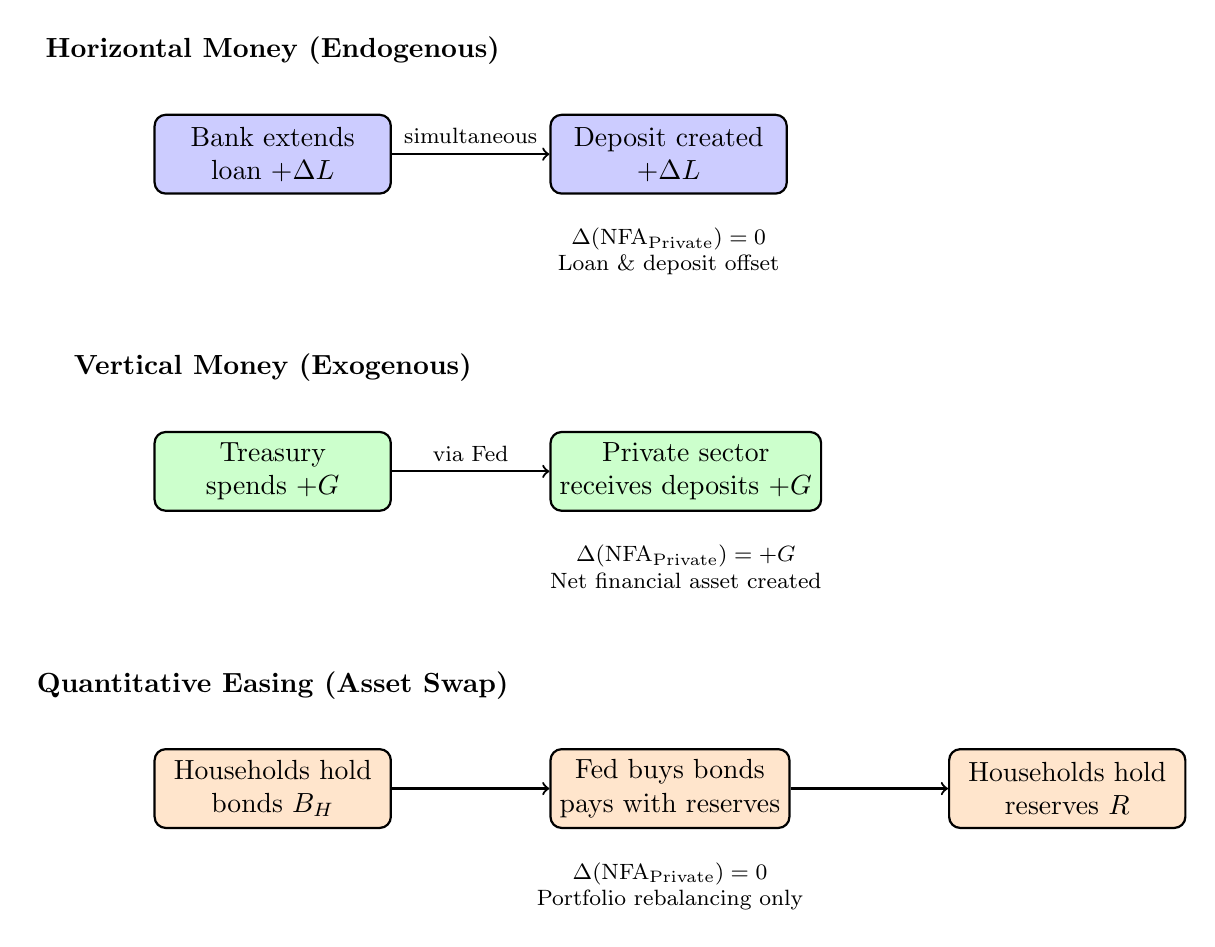
\begin{tikzpicture}[
    node distance=1.5cm and 2cm,
    process/.style={rectangle, rounded corners, draw=black, thick, minimum width=3cm, minimum height=1cm, align=center},
    flow/.style={->, thick},
    label/.style={font=\small}
]

% Horizontal Money Flow
\node[process, fill=blue!20] (bankloan) {Bank extends\\loan $+\Delta L$};
\node[process, fill=blue!20, right=of bankloan] (depositcreate) {Deposit created\\$+\Delta L$};
\node[label, above=0.5cm of bankloan, font=\bfseries] {Horizontal Money (Endogenous)};
\draw[flow] (bankloan) -- (depositcreate) node[midway, above, font=\footnotesize] {simultaneous};
\node[below=0.3cm of depositcreate, font=\footnotesize, align=center] {$\Delta(\NFA_{\text{Private}}) = 0$\\Loan \& deposit offset};

% Vertical Money Flow
\node[process, fill=green!20, below=3cm of bankloan] (treasury) {Treasury\\spends $+G$};
\node[process, fill=green!20, right=of treasury] (privatesector) {Private sector\\receives deposits $+G$};
\node[label, above=0.5cm of treasury, font=\bfseries] {Vertical Money (Exogenous)};
\draw[flow] (treasury) -- (privatesector) node[midway, above, font=\footnotesize] {via Fed};
\node[below=0.3cm of privatesector, font=\footnotesize, align=center] {$\Delta(\NFA_{\text{Private}}) = +G$\\Net financial asset created};

% QE Operation
\node[process, fill=orange!20, below=3cm of treasury] (qe1) {Households hold\\bonds $B_H$};
\node[process, fill=orange!20, right=of qe1] (qe2) {Fed buys bonds\\pays with reserves};
\node[process, fill=orange!20, right=of qe2] (qe3) {Households hold\\reserves $R$};
\node[label, above=0.5cm of qe1, font=\bfseries] {Quantitative Easing (Asset Swap)};
\draw[flow] (qe1) -- (qe2);
\draw[flow] (qe2) -- (qe3);
\node[below=0.3cm of qe2, font=\footnotesize, align=center] {$\Delta(\NFA_{\text{Private}}) = 0$\\Portfolio rebalancing only};

\end{tikzpicture}
}%
\caption{Three types of monetary operations. Horizontal money (bank lending) creates offsetting assets and liabilities. Vertical money (fiscal operations) changes private net financial assets. QE/QT are portfolio swaps that preserve private net financial assets.}
\label{fig:operations}
\end{figure}

% Multi-period dynamics figures
\begin{figure}[htbp]
\centering
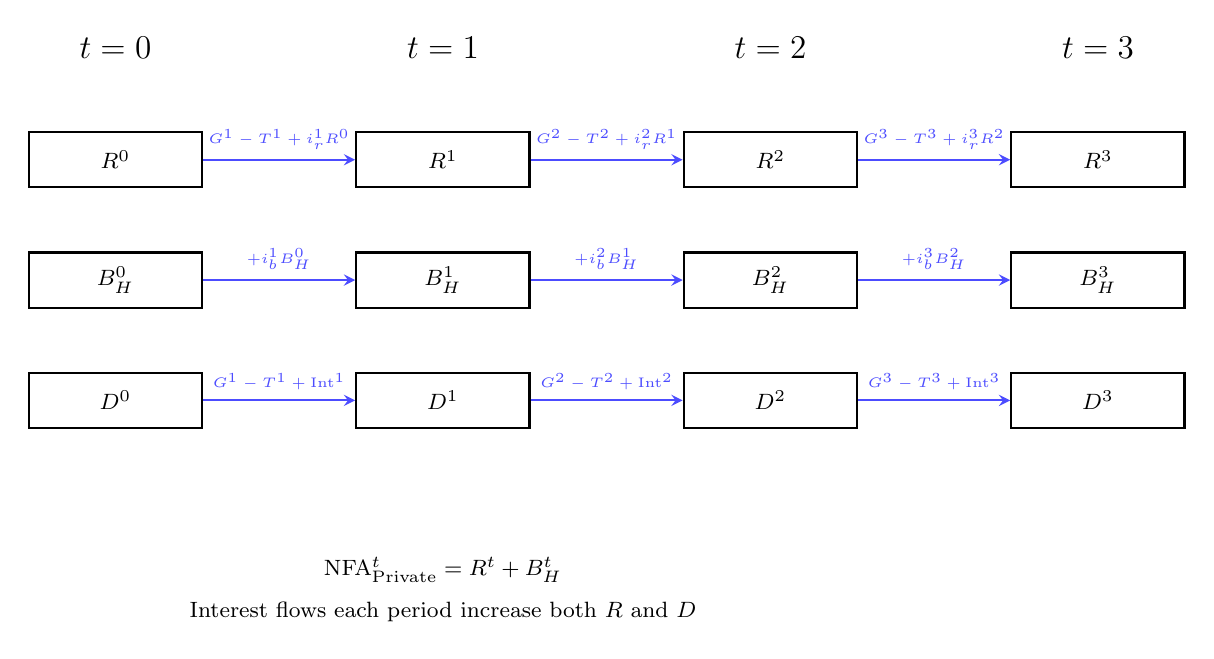
\begin{tikzpicture}[
    node distance=0.8cm and 3cm,
    stock/.style={rectangle, draw=black, thick, minimum width=2.2cm, minimum height=0.7cm, align=center, font=\footnotesize},
    flow/.style={->, thick, >=stealth},
    time/.style={font=\bfseries\large}
]

% Period t=0
\node[time] (t0) {$t=0$};
\node[stock, below=of t0] (r0) {$R^0$};
\node[stock, below=of r0] (bh0) {$B_H^0$};
\node[stock, below=of bh0] (d0) {$D^0$};

% Period t=1
\node[time, right=of t0] (t1) {$t=1$};
\node[stock, below=of t1] (r1) {$R^1$};
\node[stock, below=of r1] (bh1) {$B_H^1$};
\node[stock, below=of bh1] (d1) {$D^1$};

% Period t=2
\node[time, right=of t1] (t2) {$t=2$};
\node[stock, below=of t2] (r2) {$R^2$};
\node[stock, below=of r2] (bh2) {$B_H^2$};
\node[stock, below=of bh2] (d2) {$D^2$};

% Period t=3
\node[time, right=of t2] (t3) {$t=3$};
\node[stock, below=of t3] (r3) {$R^3$};
\node[stock, below=of r3] (bh3) {$B_H^3$};
\node[stock, below=of bh3] (d3) {$D^3$};

% Flow arrows with interest
\draw[flow, blue!70] (r0.east) -- (r1.west) node[midway, above, font=\tiny] {$G^1 - T^1 + i_r^1 R^0$};
\draw[flow, blue!70] (bh0.east) -- (bh1.west) node[midway, above, font=\tiny] {$+ i_b^1 B_H^0$};
\draw[flow, blue!70] (d0.east) -- (d1.west) node[midway, above, font=\tiny] {$G^1 - T^1 + \text{Int}^1$};

\draw[flow, blue!70] (r1.east) -- (r2.west) node[midway, above, font=\tiny] {$G^2 - T^2 + i_r^2 R^1$};
\draw[flow, blue!70] (bh1.east) -- (bh2.west) node[midway, above, font=\tiny] {$+ i_b^2 B_H^1$};
\draw[flow, blue!70] (d1.east) -- (d2.west) node[midway, above, font=\tiny] {$G^2 - T^2 + \text{Int}^2$};

\draw[flow, blue!70] (r2.east) -- (r3.west) node[midway, above, font=\tiny] {$G^3 - T^3 + i_r^3 R^2$};
\draw[flow, blue!70] (bh2.east) -- (bh3.west) node[midway, above, font=\tiny] {$+ i_b^3 B_H^2$};
\draw[flow, blue!70] (d2.east) -- (d3.west) node[midway, above, font=\tiny] {$G^3 - T^3 + \text{Int}^3$};

% NFA box
\node[below=1.5cm of d1, align=center, font=\footnotesize] (nfa) {
    $\NFA^t_{\text{Private}} = R^t + B_H^t$ \\[0.2cm]
    Interest flows each period increase both $R$ and $D$
};

\end{tikzpicture}
\caption{Multi-period stock evolution with interest payments. Each period, interest accrues on beginning-of-period stocks $(R^{t-1}, B_H^{t-1})$ and flows into reserves and deposits. Private net financial assets $\NFA^t = R^t + B_H^t$ grow by the nominal deficit.}
\label{fig:multiperiod-stocks}
\end{figure}

\begin{figure}[htbp]
\centering
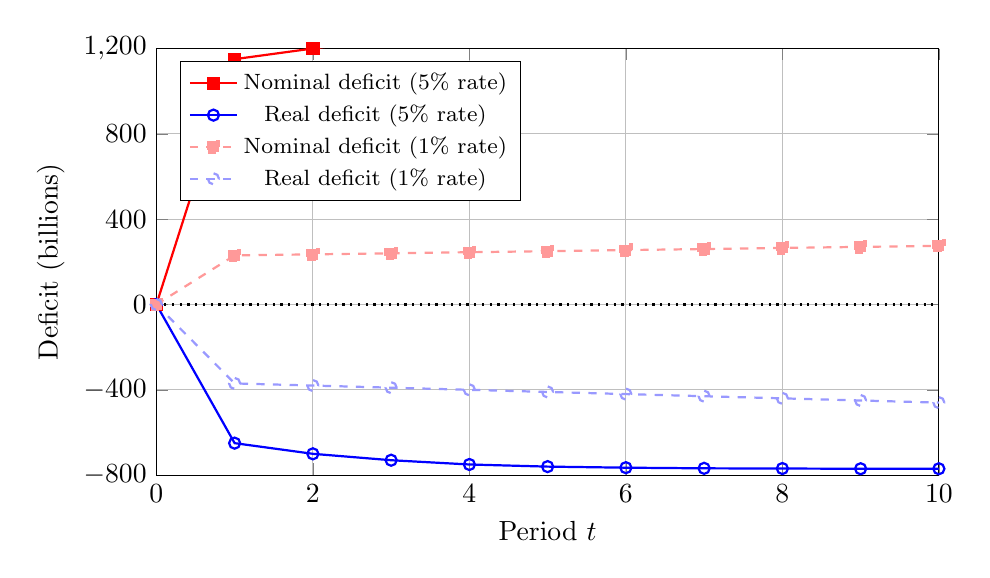
\begin{tikzpicture}
\begin{axis}[
    width=0.95\textwidth,
    height=7cm,
    xlabel={Period $t$},
    ylabel={Deficit (billions)},
    legend pos=north west,
    grid=major,
    xmin=0, xmax=10,
    ymin=-800, ymax=1200,
    xtick={0,2,4,6,8,10},
    ytick={-800,-400,0,400,800,1200},
    legend style={font=\footnotesize},
    every axis plot/.append style={thick}
]

% Nominal deficit - rate hike scenario (5% rate)
\addplot[color=red, mark=square*] coordinates {
    (0,0) (1,1150) (2,1200) (3,1250) (4,1300) (5,1350) (6,1400) (7,1450) (8,1500) (9,1550) (10,1600)
};
\addlegendentry{Nominal deficit (5\% rate)}

% Real deficit - rate hike scenario
\addplot[color=blue, mark=o] coordinates {
    (0,0) (1,-650) (2,-700) (3,-730) (4,-750) (5,-760) (6,-765) (7,-768) (8,-769) (9,-770) (10,-770)
};
\addlegendentry{Real deficit (5\% rate)}

% Nominal deficit - low rate scenario (1% rate)
\addplot[color=red!40, mark=square*, dashed] coordinates {
    (0,0) (1,230) (2,235) (3,240) (4,245) (5,250) (6,255) (7,260) (8,265) (9,270) (10,275)
};
\addlegendentry{Nominal deficit (1\% rate)}

% Real deficit - low rate scenario
\addplot[color=blue!40, mark=o, dashed] coordinates {
    (0,0) (1,-370) (2,-380) (3,-390) (4,-400) (5,-410) (6,-420) (7,-430) (8,-440) (9,-450) (10,-460)
};
\addlegendentry{Real deficit (1\% rate)}

\draw[dotted, thick] (axis cs:0,0) -- (axis cs:10,0);

\end{axis}
\end{tikzpicture}
\caption{Multi-period nominal vs.\ real deficit trajectories under high-debt scenario (120\% debt/GDP). Rate hike from 1\% to 5\% increases nominal deficit sharply (via interest payments) but produces \emph{larger real surplus} due to inflation erosion. Illustrates Mosler's deficit channel: rate hikes can be inflationary when debt is high.}
\label{fig:deficit-trajectories}
\end{figure}


\section{The Sectoral Balance Identity (Closed Economy)}

\begin{theorem}[Financial Sectoral Balance Identity]
\label{thm:sectoral-balance}
In this four-sector closed-economy model,
\[
\NFA_{\text{Private}} = R + B_H = -(NW_T + NW_{CB}).
\]
Equivalently, the consolidated public sector's (financial) net worth is the negative of the private sector's net financial assets.
\end{theorem}

\begin{proof}
Write the relevant balance sheets using only the instruments in Section 2.

\textbf{Treasury:} assets $\TGA$; liabilities $B_H + B_F$:
\[
NW_T = \TGA - (B_H + B_F).
\]

\textbf{Central bank:} assets $B_F$; liabilities $R + \TGA$:
\[
NW_{CB} = B_F - (R + \TGA).
\]

Consolidate:
\begin{align*}
NW_T + NW_{CB}
&= \bigl(\TGA - (B_H + B_F)\bigr) + \bigl(B_F - (R + \TGA)\bigr) \\
&= - (R + B_H).
\end{align*}
Rearranging yields $R + B_H = -(NW_T + NW_{CB})$, which is exactly the claim.
\end{proof}

\begin{remark}
This is pure accounting: it is true \emph{by construction} given the sector definitions and the instrument list. It does not depend on behavioral assumptions (preferences, investment functions, etc.).
\end{remark}

\section{Monetary Operations}

Figure \ref{fig:operations} summarizes the three broad classes of operations discussed below.

\subsection{Horizontal Money: Bank Credit}

\begin{definition}[Horizontal Money]
\emph{Horizontal money} refers to private credit creation inside the private sector (banks and households). It expands gross balance sheets but does not change private net financial assets.
\end{definition}

\begin{proposition}[Loan Creates Matching Deposit]
\label{prop:credit-expansion}
If banks extend new credit $\Delta L>0$ to households, then deposits rise by the same amount $\Delta D = \Delta L$. In particular,
\[
\Delta \NFA_{\text{Private}} = \Delta(R + B_H) = 0.
\]
\end{proposition}

\begin{proof}
In the stylized single-bank case (used by the interactive application), the new loan appears as a bank asset and a household liability; the matching deposit appears as a household asset and a bank liability:
\[
\Delta L = +\Delta L,\quad \Delta D = +\Delta L,
\]
with no direct change in $R$, $B_H$, $B_F$, or $\TGA$. Therefore $\Delta(R + B_H)=0$.
\end{proof}

\begin{remark}
In multi-bank settings, payments and clearing can move reserves between banks \emph{after} lending. That affects reserve \emph{distribution}, not the accounting fact that lending creates a deposit and loan simultaneously.
\end{remark}

\begin{corollary}[``Loanable Funds'' Fails as Accounting]
The statement ``banks lend out deposits'' is not a balance sheet description of lending. In the act of lending, the deposit is created; it is not a pre-existing stock that must be gathered first.
\end{corollary}

\subsection{Vertical Money: Fiscal Spending and Taxes}

\begin{definition}[Vertical Money]
\emph{Vertical money} refers to changes in the private sector's net position against the public sector caused by fiscal operations (spending and taxes).
\end{definition}

\begin{proposition}[Treasury Spending Adds Private Net Financial Assets]
\label{prop:fiscal-spend}
When the Treasury spends $G>0$ into the household sector (with banks as the settlement layer),
\[
\Delta R = +G,\qquad \Delta D = +G,\qquad \Delta \TGA = -G,
\]
and therefore $\Delta \NFA_{\text{Private}} = +G$.
\end{proposition}

\begin{proof}
The operational sequence is:
\begin{enumerate}
    \item The central bank reduces the Treasury's deposit ($\TGA$) and increases bank reserves $R$ by $G$ (a shift within central bank liabilities).
    \item Banks credit household deposits $D$ by $G$ and receive $G$ more reserves.
\end{enumerate}
Thus $R$ rises and $B_H$ is unchanged, so $\Delta(R+B_H)=+G$.
\end{proof}

\begin{proposition}[Taxes Drain Private Net Financial Assets]
\label{prop:tax}
When taxes of amount $T>0$ are paid from deposits,
\[
\Delta R = -T,\qquad \Delta D = -T,\qquad \Delta \TGA = +T,
\]
and therefore $\Delta \NFA_{\text{Private}} = -T$.
\end{proposition}

\begin{proof}
Tax payment debits household deposits and transfers reserves from banks to the central bank while increasing the Treasury's account:
bank reserves fall by $T$ and $B_H$ is unchanged, so $\Delta(R+B_H)=-T$.
\end{proof}

\begin{corollary}[Deficit Equals Change in Private Net Financial Assets]
\label{cor:deficit}
In this closed-economy, no-interest toy model, the fiscal balance determines the change in private net financial assets:
\[
\Delta \NFA_{\text{Private}} = \Delta(R+B_H) = G - T.
\]
\end{corollary}

\subsection{Treasury Securities: Reserve Drains (Not ``Funding'')}

\begin{proposition}[Bond Issuance Is a Portfolio Swap]
\label{prop:bond-issue}
When the Treasury issues $B>0$ of securities to households, paying with deposits,
\[
\Delta B_H = +B,\qquad \Delta R = -B,\qquad \Delta D = -B,\qquad \Delta \TGA = +B,
\]
and therefore $\Delta \NFA_{\text{Private}} = \Delta(R+B_H)=0$.
\end{proposition}

\begin{proof}
Households exchange deposits for a Treasury security: $D$ falls and $B_H$ rises.
Settlement drains reserves from banks ($R$ falls) and credits the Treasury's account ($\TGA$ rises). Netting $R$ and $B_H$ shows no change in $\NFA_{\text{Private}}$:
\[
(R-B) + (B_H + B) = R + B_H.
\]
\end{proof}

\begin{remark}
Operationally, Treasury issuance is often paired with spending under current U.S.\ institutional rules (the Treasury spends from the $\TGA$). In accounting terms, issuance is best viewed as a reserve drain / asset swap that supports interest-rate implementation, not as a mechanism that provides the government with something it otherwise ``lacks'' in its own unit of account.
\end{remark}

\subsection{QE and QT: Central Bank Asset Swaps}

\begin{proposition}[QE Preserves Private Net Financial Assets]
\label{prop:qe}
Under quantitative easing (QE), the central bank purchases $Q>0$ of Treasury securities from households:
\[
\Delta B_H = -Q,\qquad \Delta B_F = +Q,\qquad \Delta R = +Q,\qquad \Delta D = +Q,
\]
and therefore $\Delta \NFA_{\text{Private}} = 0$.
\end{proposition}

\begin{proof}
QE swaps a Treasury security held by households for reserve-backed bank deposits. In this model, reserves rise by $Q$ and household bond holdings fall by $Q$, so $R+B_H$ is unchanged.
\end{proof}

\begin{proposition}[QT Is the Reverse Swap]
Under quantitative tightening (QT), the central bank sells $Q>0$ of its Treasury securities to households:
\[
\Delta B_H = +Q,\qquad \Delta B_F = -Q,\qquad \Delta R = -Q,\qquad \Delta D = -Q,
\]
and therefore $\Delta \NFA_{\text{Private}} = 0$.
\end{proposition}

\begin{remark}
These are \emph{nominal} accounting statements. QE/QT can still have valuation and distributional effects (e.g.\ via term premia, risk appetite, and asset prices). Those channels are outside the scope of this balance-sheet-only model.
\end{remark}

\subsection{Summary Table (What Changes, What Doesn't)}

Table \ref{tab:summary} records the stock changes posted by the interactive application for each operation.

\begin{table}[htbp]
\centering
\begin{tabular}{@{}lrrrrrr@{}}
\toprule
Operation & $\Delta D$ & $\Delta L$ & $\Delta R$ & $\Delta B_H$ & $\Delta B_F$ & $\Delta \TGA$ \\
\midrule
Bank credit ($+\Delta L$) & $+\Delta L$ & $+\Delta L$ & $0$ & $0$ & $0$ & $0$ \\
Spend ($+G$) & $+G$ & $0$ & $+G$ & $0$ & $0$ & $-G$ \\
Tax ($+T$) & $-T$ & $0$ & $-T$ & $0$ & $0$ & $+T$ \\
Bond issue ($+B_H$) & $-B$ & $0$ & $-B$ & $+B$ & $0$ & $+B$ \\
QE ($+B_F$) & $+Q$ & $0$ & $+Q$ & $-Q$ & $+Q$ & $0$ \\
QT ($-B_F$) & $-Q$ & $0$ & $-Q$ & $+Q$ & $-Q$ & $0$ \\
\bottomrule
\end{tabular}
\caption{Stock changes posted by each operation. Only fiscal deficits/surpluses change $\NFA_{\text{Private}}=R+B_H$. Bank credit expands gross balance sheets (loans and deposits) without changing $\NFA_{\text{Private}}$.}
\label{tab:summary}
\end{table}

\section{Implications (and What This Does \emph{Not} Claim)}

\subsection{What Follows Immediately}

From the propositions above:
\begin{itemize}
    \item Bank lending is not constrained by a pre-existing stock of deposits as a matter of double-entry bookkeeping (Proposition \ref{prop:credit-expansion}).
    \item In this closed-economy model, fiscal deficits add net financial assets to the private sector (Corollary \ref{cor:deficit}).
    \item Bond issuance and QE/QT preserve private net financial assets and therefore cannot, \emph{as accounting operations}, be described as changing ``private net wealth'' (Propositions \ref{prop:bond-issue} and \ref{prop:qe}).
\end{itemize}

\subsection{What Requires Additional Economics}

This document does not, by itself, answer questions about inflation, real resource constraints, growth, distribution, or financial stability. Those require behavioral relationships, institutional detail, and (often) a richer sectoral breakdown.

\section{Connection to the Interactive Application}

The web application (\texttt{src/App.jsx}) implements the same stock variables and operations:
\begin{itemize}
    \item Stocks: \texttt{deposits}$\leftrightarrow D$, \texttt{loans}$\leftrightarrow L$, \texttt{reserves}$\leftrightarrow R$, \texttt{bondsHouseholds}$\leftrightarrow B_H$, \texttt{bondsCb}$\leftrightarrow B_F$, \texttt{tga}$\leftrightarrow \TGA$.
    \item Identity check: \texttt{privateNfw} $= R + B_H$ and \texttt{publicNetWorth} $= NW_T + NW_{CB}$ (Theorem \ref{thm:sectoral-balance}).
    \item Optional ``TGA targeting'' logic: automatic bond issuance/redemption to keep $\TGA$ near a chosen level (a simplified reserve-management story).
\end{itemize}

\section{Multi-Period Dynamics and Interest Rate Channels}
\label{sec:multiperiod}

\subsection{Time-Indexed Stock Variables}

We now extend the static model to discrete time periods $t \in \{0,1,2,\ldots,T\}$. All stock variables are now time-indexed:
\begin{align}
D^t &\defeq \text{Deposits at end of period } t \\
L^t &\defeq \text{Loans at end of period } t \\
R^t &\defeq \text{Reserves at end of period } t \\
B_H^t &\defeq \text{Treasury securities held by households at end of period } t \\
B_F^t &\defeq \text{Treasury securities held by central bank at end of period } t \\
\TGA^t &\defeq \text{Treasury General Account at end of period } t
\end{align}

\begin{definition}[Multi-Period Net Financial Assets]
Private net financial assets at the end of period $t$ are
\[
\NFA^t_{\text{Private}} \defeq R^t + B_H^t.
\]
\end{definition}

\subsection{Interest Payments as Flow Variables}

Let $i_r^t$ denote the interest rate paid on reserves during period $t$, and $i_b^t$ the interest rate on Treasury securities. Total interest payments from the public sector to the private sector during period $t$ are:
\begin{equation}
\label{eq:interest-flows}
\text{Interest}^t = i_r^t \cdot R^{t-1} + i_b^t \cdot B_H^{t-1}.
\end{equation}

\begin{remark}
We assume interest accrues on beginning-of-period stocks and is paid at the end of the period. This is a discrete-time approximation; continuous-time models (Keen-style ODEs) would use differential equations.
\end{remark}

\subsection{Recursive Balance Sheet Updates}

The balance sheets evolve according to:
\begin{align}
D^t &= D^{t-1} + \text{Spending}^t - \text{Taxes}^t + \text{Interest}^t + \text{(other flows)} \label{eq:deposits-recursive} \\
R^t &= R^{t-1} + \text{Spending}^t - \text{Taxes}^t + \text{Interest}^t + \text{(bond ops, QE/QT)} \label{eq:reserves-recursive}
\end{align}

\begin{proposition}[Interest Payments Increase Nominal Deficit]
\label{prop:interest-deficit}
Holding primary spending and taxes fixed, an increase in interest rates $i_r$ or $i_b$ mechanically increases the nominal fiscal deficit through the interest channel:
\[
\text{Nominal Deficit}^t = (G^t + \text{Interest}^t) - T^t.
\]
When debt stocks are large relative to GDP, this interest component can dominate.
\end{proposition}

\subsection{Real vs.\ Nominal Deficits}

\begin{definition}[Real Deficit]
Let $\pi^t$ denote the inflation rate during period $t$. The \emph{real deficit} adjusts for the erosion of the real value of outstanding debt:
\[
\text{Real Deficit}^t \defeq \text{Nominal Deficit}^t - \pi^t \cdot (R^{t-1} + B_H^{t-1} + B_F^{t-1}).
\]
\end{definition}

\begin{remark}[Mosler's Observation]
Warren Mosler has emphasized that when debt/GDP ratios are high and interest payments constitute a large share of government spending, \emph{raising} interest rates can be \emph{inflationary} via the deficit channel: higher $i$ increases nominal deficits, which (if accommodated) adds spending power to the private sector. Conversely, \emph{lowering} rates may reduce inflationary pressure by shrinking the deficit.

This stands in contrast to the conventional wisdom that higher rates are always disinflationary. The channel depends critically on the \emph{real} deficit response, not just nominal interest costs.
\end{remark}

\subsection{Period-by-Period Balance Sheet Matrices}

Define the state vector at the end of period $t$ as
\[
\mathbf{X}^t \defeq \begin{pmatrix} D^t \\ R^t \\ B_H^t \\ B_F^t \\ \TGA^t \end{pmatrix}.
\]

Figure \ref{fig:multiperiod-stocks} illustrates how stocks evolve across multiple periods with interest payments flowing into reserves and deposits each period.

Flow variables during period $t$ include primary spending $G^t$, taxes $T^t$, and interest payments:
\begin{align}
\text{Interest}_r^t &= i_r^t \cdot R^{t-1}, \label{eq:int-reserves} \\
\text{Interest}_b^t &= i_b^t \cdot B_H^{t-1}, \label{eq:int-bonds-hh} \\
\text{Total Interest}^t &= \text{Interest}_r^t + \text{Interest}_b^t. \label{eq:total-int}
\end{align}

\begin{proposition}[Balance Sheet Evolution with Interest]
\label{prop:multiperiod-evolution}
Assuming no bond operations or QE/QT during period $t$, the balance sheets update as:
\begin{align}
D^t &= D^{t-1} + G^t - T^t + \text{Total Interest}^t, \label{eq:d-update} \\
R^t &= R^{t-1} + G^t - T^t + \text{Total Interest}^t, \label{eq:r-update} \\
B_H^t &= B_H^{t-1}, \label{eq:bh-update} \\
B_F^t &= B_F^{t-1}, \label{eq:bf-update} \\
\TGA^t &= \TGA^{t-1} - G^t + T^t - \text{Total Interest}^t. \label{eq:tga-update}
\end{align}
\end{proposition}

\begin{proof}
Interest payments are fiscal expenditures settled the same way as primary spending $G$: the central bank credits bank reserves and bank deposits rise. Thus equations \eqref{eq:d-update} and \eqref{eq:r-update} combine primary balance $(G^t - T^t)$ with interest. The TGA account drains by the same total in equation \eqref{eq:tga-update}.
\end{proof}

\subsection{Nominal Deficit Dynamics}

\begin{definition}[Nominal Fiscal Deficit]
The nominal deficit in period $t$ is
\[
\text{Deficit}_{\text{nom}}^t \defeq G^t + \text{Total Interest}^t - T^t.
\]
\end{definition}

\begin{proposition}[Interest Rate Hikes Amplify Nominal Deficits]
\label{prop:rate-hike-nominal}
For fixed primary balance $G^t - T^t$ and debt stocks $(R^{t-1}, B_H^{t-1})$, the partial derivative of the nominal deficit with respect to the interest rate is
\[
\frac{\partial \text{Deficit}_{\text{nom}}^t}{\partial i_r^t} = R^{t-1}, \quad
\frac{\partial \text{Deficit}_{\text{nom}}^t}{\partial i_b^t} = B_H^{t-1}.
\]
When debt stocks are large (e.g.\ $R + B_H \gg$ annual GDP), a 1 percentage point rate increase produces a large absolute increase in nominal spending.
\end{proposition}

\begin{proof}
Direct differentiation of $\text{Deficit}_{\text{nom}}^t = G^t + i_r^t R^{t-1} + i_b^t B_H^{t-1} - T^t$ with respect to $i_r^t$ and $i_b^t$ yields the stated partials.
\end{proof}

\subsection{Real Deficit and the Inflation Feedback}

\begin{definition}[Debt-to-GDP Ratio]
Let $Y^t$ denote nominal GDP in period $t$. Define
\[
d^t \defeq \frac{R^t + B_H^t + B_F^t}{Y^t}.
\]
\end{definition}

Recall from equation \eqref{eq:interest-flows} that the real deficit subtracts inflation-induced erosion of real debt value:
\[
\text{Deficit}_{\text{real}}^t = \text{Deficit}_{\text{nom}}^t - \pi^t \cdot (R^{t-1} + B_H^{t-1} + B_F^{t-1}).
\]

\begin{proposition}[Paradoxical Real Deficit Response]
\label{prop:paradox}
Suppose inflation $\pi^t$ responds positively to the nominal deficit (a standard Phillips-curve-like relationship). Then when the debt stock $R^{t-1} + B_H^{t-1} + B_F^{t-1}$ is large, a rate hike can \emph{reduce} the real deficit even as it increases the nominal deficit, if the induced inflation increase is strong enough.

Formally, if
\[
\frac{d\pi^t}{di^t} \cdot (R^{t-1} + B_H^{t-1} + B_F^{t-1}) > R^{t-1} + B_H^{t-1},
\]
then $\frac{d \text{Deficit}_{\text{real}}^t}{di^t} < 0$.
\end{proposition}

\begin{proof}
Differentiate the real deficit with respect to the average interest rate $i^t$ (assuming $i_r^t \approx i_b^t \approx i^t$ for simplicity):
\begin{align*}
\frac{d \text{Deficit}_{\text{real}}^t}{di^t}
&= \frac{d \text{Deficit}_{\text{nom}}^t}{di^t} - \frac{d\pi^t}{di^t} \cdot (R^{t-1} + B_H^{t-1} + B_F^{t-1}) \\
&= (R^{t-1} + B_H^{t-1}) - \frac{d\pi^t}{di^t} \cdot (R^{t-1} + B_H^{t-1} + B_F^{t-1}).
\end{align*}
If $\frac{d\pi^t}{di^t}$ is large enough (i.e., deficit spending is highly inflationary and debt is large), the second term dominates and the derivative is negative.
\end{proof}

\begin{remark}[Mosler's Insight]
This formalizes Mosler's observation: when debt/GDP is high, rate hikes add so much nominal spending via interest that inflation rises enough to erode real debt value faster than the nominal deficit increases. The net effect can be a \emph{lower} real deficit and \emph{higher} inflation, opposite to conventional monetary policy expectations \cite{bloomberg2024}.
\end{remark}

\subsection{Numerical Example: High Debt Scenario}

Consider a stylized economy with:
\begin{align*}
Y^0 &= 25{,}000 \text{ billion (GDP)}, \\
R^0 &= 3{,}000, \quad B_H^0 = 20{,}000, \quad B_F^0 = 7{,}000, \\
d^0 &= \frac{30{,}000}{25{,}000} = 1.2 \text{ (debt/GDP = 120\%)}.
\end{align*}

Assume primary balance is zero: $G^t - T^t = 0$ for all $t$.

\textbf{Scenario A (Low rates):} $i^t = 1\%$.
\[
\text{Interest}^1 = 0.01 \cdot 23{,}000 = 230.
\]
If this produces $\pi^1 = 2\%$, then
\[
\text{Deficit}_{\text{real}}^1 = 230 - 0.02 \cdot 30{,}000 = 230 - 600 = -370 \text{ (real surplus)}.
\]

\textbf{Scenario B (High rates):} $i^t = 5\%$.
\[
\text{Interest}^1 = 0.05 \cdot 23{,}000 = 1{,}150.
\]
If this produces $\pi^1 = 6\%$ (higher deficit $\Rightarrow$ higher inflation), then
\[
\text{Deficit}_{\text{real}}^1 = 1{,}150 - 0.06 \cdot 30{,}000 = 1{,}150 - 1{,}800 = -650 \text{ (larger real surplus)}.
\]

Thus the rate hike from 1\% to 5\% increased nominal deficit by $1{,}150 - 230 = 920$ but \emph{increased} the real surplus by $650 - 370 = 280$ due to inflation erosion. This is the deficit channel in action \cite{cnbc2022,reuters2022}. Figure \ref{fig:deficit-trajectories} visualizes these divergent trajectories over multiple periods.

\subsection{Multi-Period Trajectories}

For $t=0,1,2,\ldots,T$, one can iterate equations \eqref{eq:d-update}--\eqref{eq:tga-update} with evolving interest rates $i^t$ and inflation $\pi^t$. The interactive application (Section \ref{sec:app-integration}) will allow users to configure scenarios and visualize:
\begin{itemize}
    \item Nominal vs.\ real deficit paths under rate hike vs.\ rate cut.
    \item Debt/GDP ratio evolution.
    \item Inflation trajectories induced by deficit feedback.
\end{itemize}

\subsection{Connection to Interactive Application}
\label{sec:app-integration}

The React application will implement a \texttt{MultiPeriodSim} component that:
\begin{itemize}
    \item Maintains state arrays for $t=0,\ldots,T$ (default $T=10$).
    \item Computes $\text{Interest}^t$, $\text{Deficit}_{\text{nom}}^t$, $\text{Deficit}_{\text{real}}^t$ each period.
    \item Updates $R^t, B_H^t, D^t$ recursively per Proposition \ref{prop:multiperiod-evolution}.
    \item Displays charts of nominal/real deficits, inflation, debt/GDP over time.
    \item Allows user to configure: initial debt/GDP, interest rate path (constant, ramp, shock), inflation elasticity.
\end{itemize}

This provides an interactive demonstration of Propositions \ref{prop:rate-hike-nominal} and \ref{prop:paradox}.

\section{References}

\begin{itemize}
    \item Godley, W., \& Lavoie, M. (2007). \textit{Monetary Economics: An Integrated Approach to Credit, Money, Income, Production and Wealth}. Palgrave Macmillan.
    \item Kelton, S. (2020). \textit{The Deficit Myth}. PublicAffairs.
    \item Keen, S. (2011). \textit{Debunking Economics}. Zed Books.
    \item Mosler, W. (various). \textit{Soft Currency Economics} and related papers.
    \item \label{reuters2022} ``Central banks will fail to tame inflation without better fiscal policy, study says,'' Reuters, August 27, 2022. \url{https://www.reuters.com/markets/us/central-banks-will-fail-tame-inflation-without-better-fiscal-policy-study-says-2022-08-27/}
    \item \label{cnbc2022} ``Joseph Stiglitz thinks further Fed rate hikes could make inflation worse,'' CNBC, September 2, 2022. \url{https://www.cnbc.com/amp/2022/09/02/joseph-stiglitz-thinks-further-fed-rate-hikes-could-make-inflation-worse.html}
    \item \label{bloomberg2024} ``Warren Mosler Explains Why High Interest Rates Might Fan Inflation,'' Bloomberg, July 9, 2024. \url{https://www.bloomberg.com/news/articles/2024-07-09/warren-mosler-explains-why-high-interest-rates-might-fan-inflation}
\end{itemize}

\end{document}
